\chapter{Game and AI Framework Implementation}

The framework in Durak is tailored to support the implementation and evaluation of artificial intelligence algorithms within the game environment. The main objective of the it is to provide a framework for the development and testing of AI agents, aiming to evaluate their performance within the game. This chapter presents a high-level overview of the game and AI framework, including its capabilities for supporting the development and evaluation of AI for Durak. 

A more in-depth analysis of the implementation and functionality of the game model can be found in section \ref{devdoc} of the developer documentation, as well as in the user documentation provided in section \ref{userdoc}. These sections provide comprehensive information on the design and implementation of the game model, as well as its capabilities and usage for both developers and end users.

\section{OS support}

The game framework for Durak was tested on both Windows 10 and Linux operating systems to confirm compatibility and functionality. While this list is not exhaustive, and the framework may potentially run on other operating systems, these are the only ones that were formally tested. It is possible that the framework will operate correctly on other platforms, but this has not been verified.

\section{Design}

The Durak AI framework includes a game model, AI agents, and a Command-Line Interface (CLI) that are implemented using the C\# programming language and targeted for the .NET Core 6 platform.

C\# was selected as the programming language for the implementation of aforementioned projects in Durak due to its suitability for writing back-end systems. The language offers a range of reliable libraries and benefits from a highly optimized Just-In-Time (JIT) compiler, resulting in enhanced speed. These attributes made C\# an ideal choice for this development.

In order to run and test the program, the project has to be cloned from the repository and opened with an Integrated Development Environment (IDE) of user's choice. From the root directory of the project, the user can utilize the command line to enter the command 
\begin{verbatim}
dotnet run --project CLI
\end{verbatim}
, which will launch the Command-Line Interface (CLI) and provide guidance on how to proceed with experimentation. The CLI will provide further instructions on how to use and test the program (for additional information, please refer to Section \ref{CLI}.).

\subsection{Project Structure}
The game Durak is organized within a solution file, with the file extension ``.sln'', which is a type of file used to manage projects in Visual Studio. This solution includes three individual projects: 

\begin{itemize}

\item Model - A C\# library project contains the game logic for Durak.

\item Agent - A C\# library contains all of the implemented AI agents.

\item CLI - A C\# Command-Line Interface (CLI) project includes parameters for modifying the game model and agents settings in order to perform experiments.

The aforementioned components will be further discussed in the following subsections.

\end{itemize}

\subsection{Game Model}

The game model, which represents the current state of the game, is implemented using object-oriented programming principles. As it was mentioned before, the game logic for Durak is contained within the \textbf{Model} C\# library, which serves as a modular and reusable unit. It includes class objects, such as Player, Card, and Deck, as well as all of the other main components that make up the game each of which is equipped with the necessary methods to support the game's functionality. These objects and their methods are designed to reflect the key components and features described in the game description.

\begin{figure}[h]
    \centering
    \captionsetup{justification=centering}
    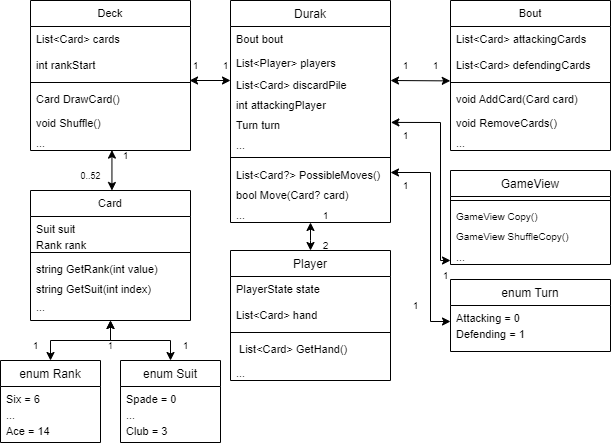
\includegraphics[width=0.9\textwidth]{../img/modelUML.png}
    \caption{A simplified UML diagram showing the relationship between the objects within the Model library.}
    \label{fig:modelUML}
\end{figure}

Before delving into the description of the game state and components of Durak, it is useful to first consider the relationship of all of the objects in the model to that state. A class diagram illustrating the relationships between the objects in the model can be found in Figure \ref{fig:modelUML}.

The representation of the game state \texttt{Durak} in the model is a key aspect of the overall system. This representation holds all of the necessary information and logic required to play the game of Durak, shown in Figure \ref{fig:codeDurak}, and therefore plays a central role in the functioning of the model. As such, it is important to carefully consider the design and implementation of the game state representation along with its components. 

\begin{figure}[h]
\captionsetup{justification=centering}
\lstset{basicstyle=\ttfamily\scriptsize}
\begin{lstlisting}[frame=single]
// Bout object of the game
private Bout bout;

// Deck object of the game
private Deck deck;

// Trump card of the game that can be assigned or not
private Card? trumpCard;

// Representation of the discard pile in the game
private List<Card> discardPile = new List<Card>();

// Players inside the game
private List<Player> players = new List<Player>();

\end{lstlisting}
\caption{A simplified diagram of the Durak class, which encompasses the main properties of the game}
\label{fig:codeDurak}
\end{figure}

The object in question serves as a comprehensive representation of all game states and data throughout a single game of Durak. Because of that it is utilized to communicate this information to other components within the system, such as the command-line interface (CLI) or artificial intelligence (AI) scripts. To facilitate communication and coordination between the Durak model and the agents that interact with it, the game state provides two primary functions: \texttt{PossibleMoves}, shown in Figure \ref{fig:codePossibleMoves} and \texttt{Move}, shown in Figure \ref{fig:codeMove}. These functions serve as the primary means through which changes can be made to the game state, and as such, play a crucial role in the overall operation of the model. 

\begin{figure}[h]
\captionsetup{justification=centering}
\lstset{basicstyle=\ttfamily\scriptsize}
\begin{lstlisting}[frame=single]

if (turn == Turn.Attacking){
	if (CanAttack() && OpponentCanFitMoreCards()) {
		return GenerateListOfAttackingCards();
	} else {
		// passing the attack
		return null;	
	}
}
else {
	Card attackingCard = bout.GetAttackingCards()[^1]
	if (CanDefend(attackingCard)) {
		return GenerateListofDefendingCards(attackingCard);
	} else {
		// taking the cards
		return null
	}
}
\end{lstlisting}
\caption{A simplified overview of the PossibleMoves method inside the Durak class}
\label{fig:codePossibleMoves}
\end{figure}

The \texttt{PossibleMoves} method determines the list of actions that are available to the current player based on the current game state and the rules of the game. When it is the attacker's turn, the method considers the rules for attacking (details in section \ref{attackconditions}) and generates a list of eligible cards that can be played or allows the player to pass if no suitable cards are available. Similarly, when it is the defender's turn (details in section \ref{BeatingRule}), the method takes into account the card being attacked and generates a list of cards that can be played to defend or offers the option to take the attack if no suitable defense is available. This enables the method to adapt to the specific circumstances of the game and provide appropriate options for the current player to make a move.

The \texttt{Move} method modifies the current game state by executing the action chosen by the current player. This move is selected by the agent, which performs calculations based on the possible moves generated by the \texttt{PossibleMoves} method. The specific nature of these calculations depends on the type of agent being used. For example, a rule-based agent may simply select the lowest value rank card, while a more sophisticated agent, such Monte-Carlo Tree Search (MCTS), may use more complex decision-making processes to determine the optimal move to make. Regardless of the type of agent being used, the \texttt{Move} method ultimately updates the game state to reflect the chosen action and advances the game to the next turn.

\begin{figure}[h]
\captionsetup{justification=centering}
\lstset{basicstyle=\ttfamily\scriptsize}
\begin{lstlisting}[frame=single]
if (turn == Turn.Attacking){
	// the attacker played a card	
	if (card is not null) {
		attacker.GetHand().Remove(card);
		bout.AddCard(card);
	} else {
		bout.RemoveCards();
		return;
	}
}
else {
	// the defender beat the attacking card
	if (card is not null){
		defender.GetHand().Remove(card);
		bout.AddCard(card);
	} else {
		FillPlayerHand(bout.GetEverything(), defender)
		return;
	}	
}
turn = turn == Turn.Attacking ? Turn.Defending : Turn.Attacking;
\end{lstlisting}
\caption{A simplified overview of the Move method inside the Durak class}
\label{fig:codeMove}
\end{figure}

Additionally, it is important to note that, for security purposes, the agents are not provided with the entire \texttt{Durak} object. Instead, they are given access to a \texttt{GameView} class representation, which allows them to obtain essential information about the current game state and make changes through the methods outlined in Figures \ref{fig:codePossibleMoves} and \ref{fig:codeMove}. This approach ensures that the agents are not able to manipulate the game in an unauthorized manner.


\subsection{CLI}
\label{CLI}

\subsection{AI Agents}

\section{Interface}
